\documentclass[a4paper, fontsize=14pt]{article}
\usepackage[T2A]{fontenc}
\usepackage{mathtools}
\usepackage[utf8]{inputenc}
\usepackage[english, russian]{babel}
\usepackage{fancyhdr}
\usepackage{graphicx}
\usepackage{gensymb}
\usepackage{floatrow}
\usepackage{titlesec}
\usepackage{lastpage}
\usepackage{float}
\usepackage{gensymb}
\usepackage{booktabs}
\usepackage{amsmath}

\pagestyle{fancy}
	\fancyhf{}
	\lhead{\hspace{1bp} Работа \textnumero 2.1.6}
	\rhead{Терехов Максим 876\hspace{1bp}}
	\cfoot{\textbf{}}
	\rfoot{\thepage\ \textnormal{из}\ \pageref{LastPage}}
	\renewcommand{\headrulewidth}{1pt}
	\renewcommand{\footrulewidth}{1pt}


%\addtolength{\hoffset}{-1.75cm}
%\addtolength{\textwidth}{3.5cm} 

%\addtolength{\voffset}{-1.5cm}
%\addtolength{\textheight}{3cm} 

\titleformat{\section}
    [block]{\normalfont\bfseries\large}{\rlap{\thesection}}{0em}
    {\vspace{-0.02\textwidth}\begin{minipage}[t]{.95\textwidth}}
[\end{minipage}]

\thispagestyle{fancy}

\begin{document}
\selectlanguage{russian}
\parindent=1cm


\huge
\centering
\textbf{Эффект Джоуля-Томсона}

\raggedright
\large
	\section*{Цель работы}
		1) Определение изменения температуры углекислого газа при протекании через малопроницаемую перегородку при разных начальных значениях давления и температуры.
		2) Вычисление по результатам опытов коэффициентов Ван-дер-Ваальса <<a>> и <<b>>.
	\section*{Оборудование}
	Термостат, трубка с пористой перегородкой, труба Дьюара, дифференциальная термопара, микровольтметр, балластный баллон, манометр.
	\section*{Экспериментальная установка}
		\begin{figure}[H]
	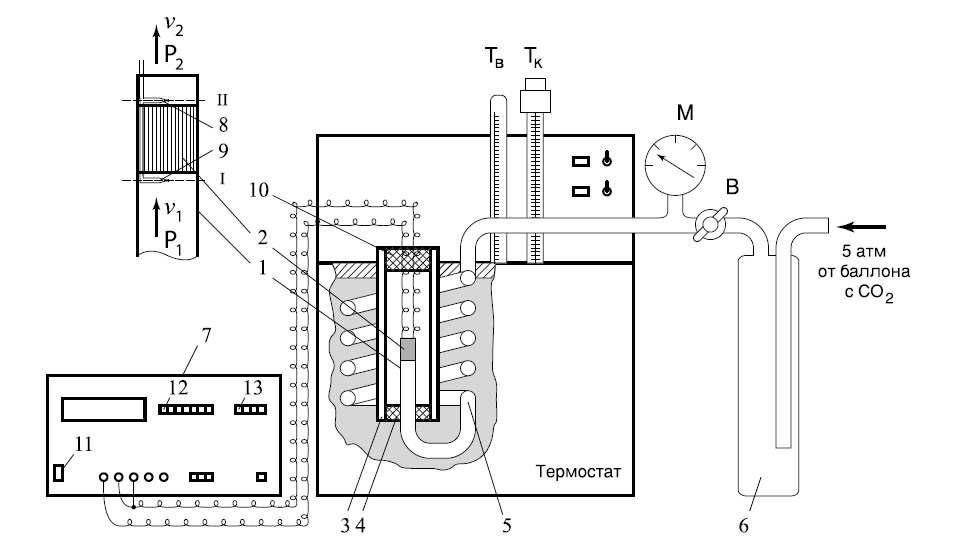
\includegraphics[width = \linewidth]{instrument}
	\end{figure}

	
	\section*{Теоретическая часть}
		Эффектом Джоуля–Томсона называется изменение температуры газа, медленно протекающего из области высокого в область низкого давления в условиях хорошей тепловой изоляции. В разреженных газах, которые приближаются по своим свойствам к идеальному газу, при таком течении температура газа не меняется. Эффект Джоуля–Томсона демонстрирует отличие исследуемого газа от идеального.

В работе исследуется изменение температуры углекислого газа при медленном его течении по трубке с пористой перегородкой. Трубка 1 хорошо теплоизолирована. Газ из области повышенного давления $P_1$ проходит через множество узких и длинных каналов пористой перегородки 2 в область с атмосферным давлением $P_2$. Перепад давления  $\Delta P = P_1 - P_2$ из-за большого сопротивления
каналов может быть заметным даже при малой скорости течения газа в трубке. Величина эффекта Джоуля–Томсона определяется по разности температуры газа до и после перегородки.

Рассмотрим стационарный поток газа между произвольными се-
чениями I и II трубки (до перегородки и после нее). Пусть, для опре-
деленности, через трубку прошел 1 моль углекислого газа; $\mu$ — его
молярная масса. Молярные объемы газа, его давления и отнесенные
к молю внутренние энергии газа в сечениях I и II обозначим соответственно $V_1$ , $P_1$, $U_1$ и $V_2$ , $P_2$ , $U_2$. Для того чтобы ввести в трубку объем $V_1$, над газом нужно совершить работу $A_1$ = $P_1 V_1$. Проходя через сечение II, газ сам совершает работу $A_2$ = $P_2$ $V_2$. Так как через боковые стенки не происходит ни обмена теплом, ни передачи механической
энергии, то
	\begin{equation}
		A_1-A_2 = \left(U_2+\frac{\mu v_2^2}{2}\right)-\left(U_1+\frac{\mu v_1^2}{2}\right).
	\end{equation}
В уравнении (1) учтено изменение как внутренней (первые члены в
скобках), так и кинетической (вторые члены в скобках) энергии газа.
Подставляя в (1) написанные выражения для $A_1$ и $A_2$ и перегруппировывая члены, найдем
	\begin{equation}
		H_1-H_2 = \left(U + P_1 V_1 \right) - \left(U_2 + P_2 V_2 \right) = \frac{1}{2}\mu\left(v_2^2-v_1^2\right)
	\end{equation}

	Сделаем несколько замечаний. Прежде всего отметим, что в процессе Джоуля–Томсона газ испытывает в пористой перегородке существенное трение, приводящее к ее нагреву. Потери энергии на нагрев трубки в начале процесса могут быть очень существенными и сильно искажают ход явления. После того как температура трубки установится и газ станет уносить с собой все выделенное им в пробке тепло, формула (1) становится точной, если, конечно, теплоизоляция трубки достаточно хороша и не происходит утечек тепла наружу через ее стенки.
	
	Второе замечание связано с правой частью (2). Процесс Джоуля–Томсона в чистом виде осуществляется лишь в том случае, если правой частью можно пренебречь, т. е. если макроскопическая скорость газа с обеих сторон трубки достаточно мала. У нас сейчас нет критерия, который позволил бы установить, когда это можно сделать. Поэтому мы отложим на некоторое время обсуждение вопроса о правой части (2), а пока будем считать, что энтальпия газа не меняется.
	
	Рассмотрим выражение:
	\begin{equation}
		\mu_{\text{Д-Т}} = \frac{\Delta T}{\Delta P} \approx \cfrac{\cfrac{2a}{RT}-b}{C_p}
	\end{equation}
	
	Из формулы (3) видно, что эффект Джоуля–Томсона для не очень
плотного газа зависит от соотношения величин $a$ и $b$, которые оказывают противоположное влияние на знак эффекта. Если силы взаимодействия между молекулами велики, так что превалирует «поправка на давление», то основную роль играет член, содержащий $a$, и
\[
	\frac{\Delta T}{\Delta P} > 0,
\]
то есть газ при расширении охлаждается ($\Delta t < 0$ так как всегда
$\Delta P < 0$). В обратном случае (малые a):
\[
	\frac{\Delta T}{\Delta P} < 0,
\]
то есть газ нагревается ($\Delta t < 0$ так как по-прежнему
$\Delta P < 0$).

Этот результат нетрудно понять из энергетических соображений.
Как мы уже знаем, у идеального газа эффект Джоуля–Томсона отсутствует. Идеальный газ отличается от реального тем, что в нем можно
пренебречь потенциальной энергией взаимодействия молекул. Наличие этой энергии приводит к охлаждению или нагреванию реальных
газов при расширении. При больших $a$ велика энергия притяжения
молекул. Это означает, что потенциальная энергия молекул при их
сближении уменьшается, а при удалении — при расширении газа ---
возрастает. Возрастание потенциальной энергии молекул происходит
за счет их кинетической энергии --- температура газа при расширении
падает. Аналогичные рассуждения позволяют понять, почему расширяющийся газ нагревается при больших значениях $b$.

Как следует из формул, при температуре $T_i$ коэффициент $\mu_\text{д-т}$ обращается в нуль. Используя связь между коэффици-
ентами $a$ и $b$ и критической температурой, найдем:
	\begin{equation}
		T_{\text{инв}}=\frac{27}{4}T_{\text{кр}}
	\end{equation}:
	
При температуре $T_\text{инв}$ эффект Джоуля–Томсона меняет знак: ниже температуры инверсии эффект положителен ($\mu_\text{д-т} > 0$, газ охлаждается), выше $T_\text{инв}$ эффект отрицателен ($\mu_\text{д-т} < 0$, газ нагревается).	
	
	
\section*{Обработка результатов измерений}

	Включим термостат и вольтметр.
	%, снимем значение поправочного напряжения: $\varepsilon_0 = 6\,\text{мкВ}$.
	Проведем измерения напряжения на термопаре и разности давлений с учетом поправочного напряженияв:\newline
	

\begin{table}[H]

	\centering
	\begin{tabular}{|c|c|c|c|c|c|c|} \hline
		$\Delta P,\ \text{атм}$ & 3.0 & 2.6 & 2.2 & 1.8 & 1.4 & 1.0 \\ \hline
		$U-U_0,\ \text{мкВ}   $ & 138 & 120 & 102 & 85 & 68 & 55 \\ \hline
		$\Delta T$, K   & 3.47 & 3.02 & 2.56 & 2.14 & 1.71 & 1.38 \\ \hline
	\end{tabular}
		\caption{T=291K}
\end{table}
\begin{table}[H]

	\centering
	\begin{tabular}{|c|c|c|c|c|c|c|} \hline
		$\Delta P,\ \text{атм}$ & 3.0 & 2.6 & 2.2 & 1.8 & 1.4 & 1.0 \\ \hline
		$U-U_0$, мкВ    & 115 & 98 & 82 & 66 & 51 & 40 \\ \hline
		$\Delta T$, K   & 2.76 & 2.36 & 1.97 & 1.59 & 1.23 & 0.96 \\ \hline
	\end{tabular}
		\caption{T=308K}
\end{table}
\begin{table}[H]
	\centering
	\begin{tabular}{|c|c|c|c|c|c|c|} \hline
		$\Delta P,\ \text{атм}$ & 3.0 & 2.6 & 2.2 & 1.8 & 1.4 & 1.0 \\ \hline
		$U-U_0$, мкВ    & 91 & 80 & 68 & 55  & 41 & 28 \\ \hline
		$\Delta T$, K   & 2.10 & 1.85 & 1.57 & 1.27 & 0.95 & 0.65 \\ \hline
	\end{tabular}
		\caption{T=333K}
\end{table}



Построим графики зависимости $\Delta T(\Delta P)$ и определим коэффициент Джоуля-Томпсона для каждой температуры:
\[
	\mu = \frac{\Delta T}{\Delta P}
\]

	\begin{figure}[H]
	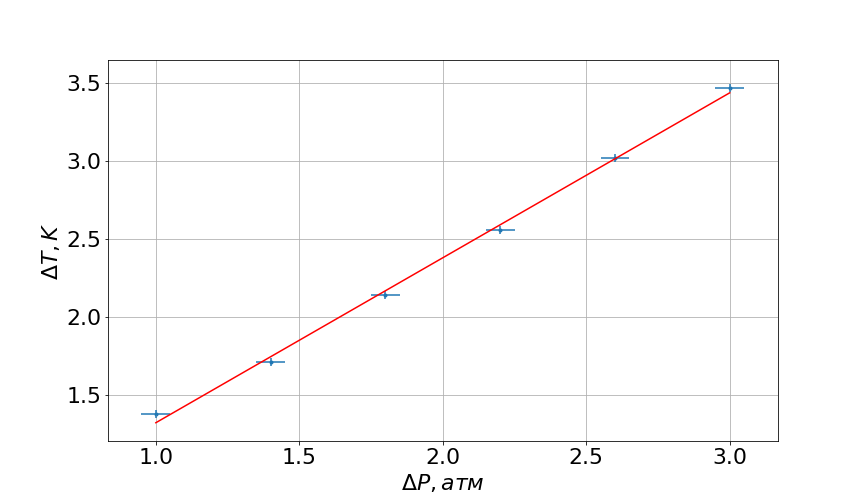
\includegraphics[width = 1.0\linewidth]{291.png}
		\caption{T = 291 K}
	\end{figure}
	
	\begin{figure}[H]
	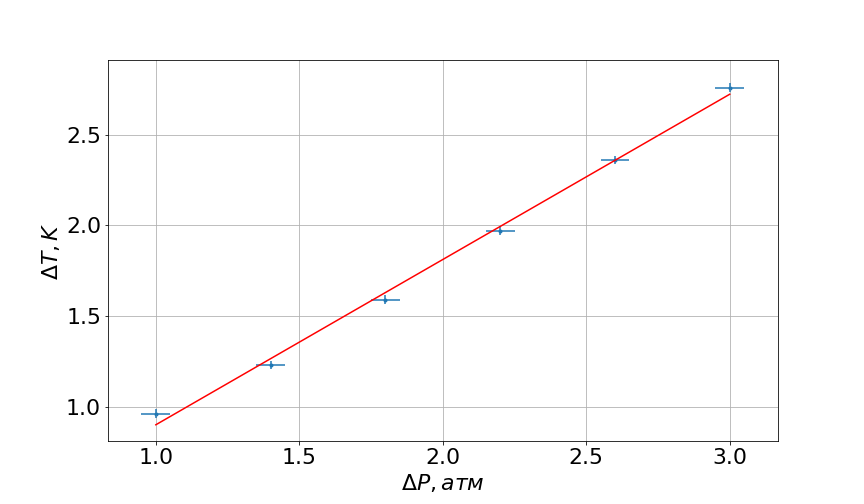
\includegraphics[width = 1.0\linewidth]{308.png}
		\caption{T = 308 K}
	\end{figure}
	
	\begin{figure}[H]
	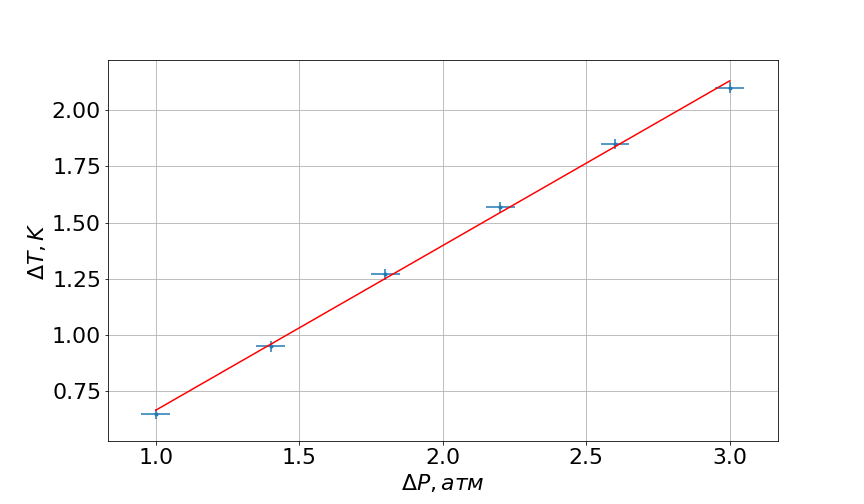
\includegraphics[width = 1.0\linewidth]{333.png}
		\caption{T = 333 K}
	\end{figure}
	
	Угловые коэффициенты графиков:
	\begin{figure}[H]
\center
\begin{tabular}{|c|c|c|}
\hline $k_1$ & $k_2$ & $k_3$ \\
\hline $1.06 \pm 0.01$ & $0.91 \pm 0.01$ & $0.73 \pm 0.01$ \\\hline
	\end{tabular}
\end{figure}


\begin{table}[H]

	\centering
	\begin{tabular}{|c|c|c|c|} \hline
		 & T = 291 K & T = 308 K & T = 333 K \\ \hline
		$\mu_{\text{Д-Т}}$ & 1.06 & 0.91 & 0.73  \\ \hline
		$\sigma_{\mu_{\text{Д-Т}}} $ & 0.01 & 0.01 & 0.01 \\ \hline
	\end{tabular}
		\caption{Коэффициенты Джоуля-Томсона}
\end{table}
Построим график зависимости $\mu$ от $1/T$:
\begin{figure}[H]
	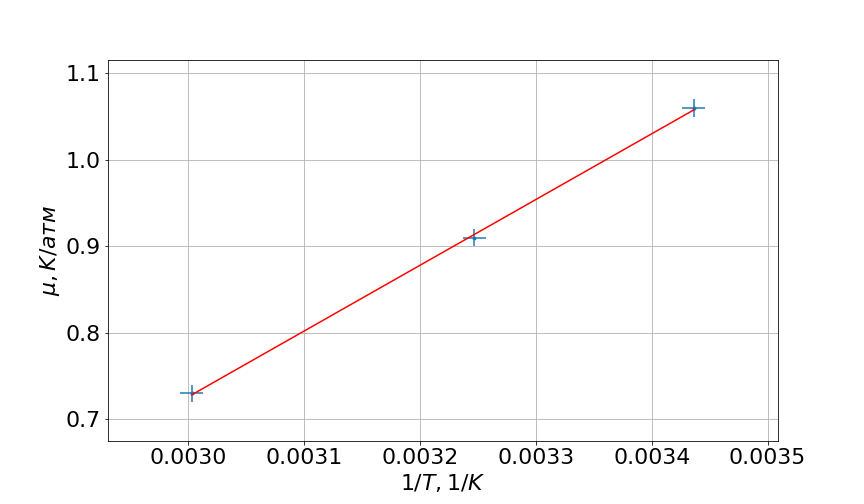
\includegraphics[width = \linewidth]{result.png}
	\caption{Зависимость $\mu$ от 1/T}
\end{figure}

Параметры графика: $K = 0.0076; \quad B = -1.555 \cdot 10^{-5}$

 
Найдём коэффициенты Ван-дер-Ваальса и температуру инверсии по коэффициенту наклона с предыдущего графика:
\[
	C_p = 41 \frac{\text{Дж}}{\text{моль} \cdot \text{К}}
\]
\[
a = \frac{KRC_p}{2} = 1.30 \pm 0.04 \frac{\text{Н}\cdot\text{м}^4}{\text{моль}^2} 
\]
\[
b = -BC_p  = (6.4 \pm 0.2)\cdot 10^{-4} \frac{\text{м}^3}{\text{моль}}.
\]
\[
	T_i = \frac{2a}{Rb} = 487 \pm 22 K
\]
Табличное значение:
\[
	T_{i_\text{табл}} = 2027 K
\]
\section*{Вывод}

Полученные экспериментальным путем значения разнятся с табличными потому, что для расчётов была использоава модель газа Ван-дер-Ваальса. Отсюда можно сделать вывод, что модель газа Ван-дер-Ваальса хорошо приближена к модели реального газа в количественном соотношении только в небольшом диапазоне.

\end{document}



